\section{Real-world Experiments}
\label{sec:real-world}

This section presents real-world experimental results validating the proposed \ac{REACT} method. The experiments were conducted at the underwater robotics facility of the German Research Center for Artificial Intelligence (DFKI), which features a $23$m$\times19$m$\times8$m test basin equipped with a 12-camera Qualisys motion capture system for precise state estimation.

\subsection{Real-world experimental setup}
The experimental platform is a BlueROV2, configured identically to the simulation setup. The test environment consists of a pipe structure with a diameter of $0.7$m and a length of $2.5$m, as shown in Fig.~\ref{fig:pipe}. Two planning modes, identical to those evaluated in simulation, are tested. The first is \ac{REACT}, which represents the full system incorporating \ac{REACT}. The second is the \ac{CPP} baseline without \ac{REACT}. In both modes, a helical trajectory is given as a reference around the pipe.

\begin{figure}[t]
    \centering
    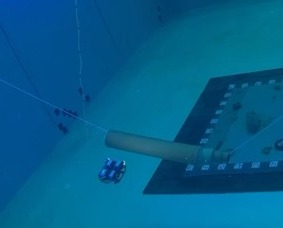
\includegraphics[width=0.65\linewidth]{figures/dfki_pipe.jpeg}
    \caption{ Experimental setup in the DFKI underwater basin showing the BlueROV2 and the test structure. The pipe is suspended horizontally in the water using cables.}
    \label{fig:pipe}
\end{figure}

\subsection{Real-world experimental results}

Real-world tests illustrate the clear benefits of the \ac{REACT} planner compared to the baseline \ac{CPP} approach. Figure~\ref{fig:realworld_trajectory} shows the mission trajectories for both methods.
As such, the baseline \ac{CPP} planner failed to complete the inspection task. At $t=124$s, the tether entangles the pipe structure, stopping the \ac{ROV} and preventing further progress. Hence, the overall coverage achieved is only $80.9\%$ (Table~\ref{tab:realworld_coverage}).




The proposed \ac{REACT} planner completed the full mission, achieving $95.6\%$ coverage. The planner adapted to tether constraints throughout the mission. Unlike the simulation results, the soft tether length limit of the $8$m was exceeded in real-world tests. As such, when no entanglement-free paths to the goal are available, \ac{REACT} treats the length constraints as a soft limit rather than a hard limitation. However, when entanglement is detected and there is an entanglement-free path around the pipe, \ac{REACT} finds a path that detangles the \ac{ROV} from the structure. This capability is demonstrated at $t = 96$s when \ac{REACT} detected an imminent tether entanglement. The planner computed a new path that safely untangled the \ac{ROV} from the pipe structure, allowing inspection to continue. The system only exceeded the soft tether limit when necessary for mission completion while prioritizing entanglement avoidance whenever possible.

The baseline \ac{CPP} planner, lacking entanglement-awareness, became permanently stuck. This demonstrates a key advantage of \ac{REACT} that was not visible in the simulation study, where the physical tether forces remain unmodeled.


Although the \ac{REACT} planner adds computation compared to the baseline, the maximum replanning time of 0.4822~s remained well within the onboard platform’s capabilities, allowing real-time operation. This overhead, while higher than the conventional \ac{CPP} approach, was low enough to enable timely adaptation to tether entanglement events.


These results demonstrate that standard planners without tether constraints fail even during relatively simple underwater 3D inspection tasks. While the baseline initially followed the planned path, it became entangled and subsequently immobilized midway through the mission. On the other hand, \ac{REACT}'s ability to detect and avoid entanglement through replanning enabled a successful mission completion. These findings highlight the need for entanglement-aware planning in real underwater operations.

\begin{table}[t]
    \centering
    \caption{Coverage Performance in Real-world Trials}
    \label{tab:realworld_coverage}
    \resizebox{0.65\columnwidth}{!}{%
    \begin{tabular}{|l|c|c|}
        \hline
        \textbf{Planner} & \textbf{Inspection Completion} & \textbf{Final Coverage (\%)} \\
        \hline
        \ac{REACT} & Full & 95.6 \\
        CPP & Failed (Entangled) & 80.9  \\
        \hline
    \end{tabular}%
    }
    \vspace{0.5em}
\end{table}

\begin{figure}[t]
    \centering
    \begin{subfigure}[b]{0.48\linewidth}
        \centering
        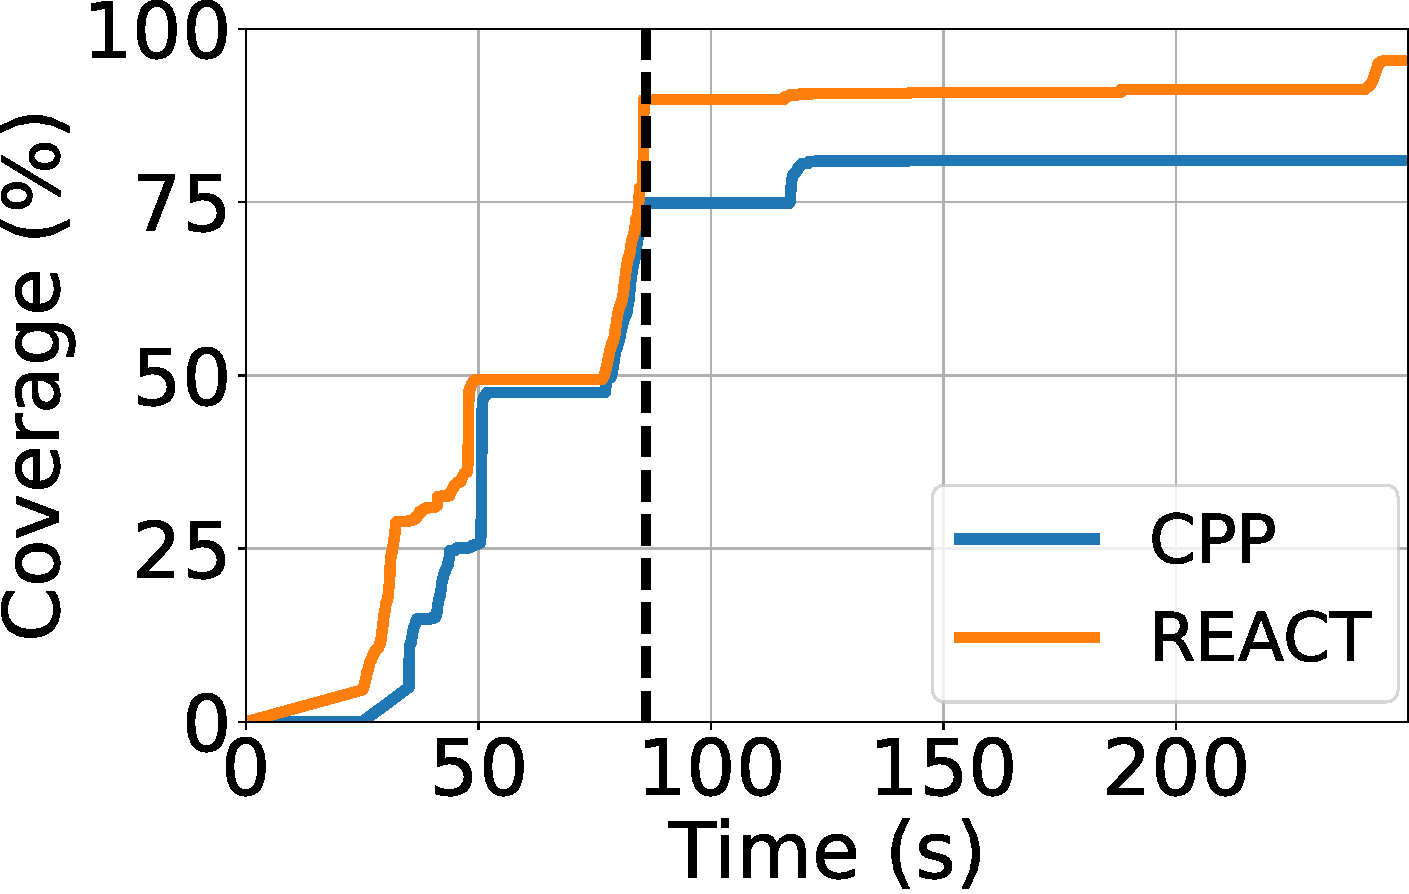
\includegraphics[width=\linewidth]{figures/coverage_comparison_plot.pdf}
        \caption{Coverage vs. time for both planners.}
        \label{fig:traj_noreact}
    \end{subfigure}
    \hfill
    \begin{subfigure}[b]{0.48\linewidth}
        \centering
        
\includegraphics[width=\linewidth]{figures/tether_length_vs_time.pdf}
        \caption{Tether length vs. time for both planners.}
        \label{fig:traj_react}
    \end{subfigure}
    \caption{Real-world ROV trajectories. Without \ac{REACT}, the mission fails due to tether entanglement. With \ac{REACT}, the ROV completes the mission successfully. At $t = 96$s, the replanner is activated, allowing \ac{REACT} to disentangle the \ac{ROV} and continue the inspection. In contrast, at $t = 124$s, the \ac{ROV} using the conventional \ac{CPP} becomes stuck due to the entangled tether.}
    \label{fig:realworld_trajectory}
\end{figure}


